% ============================================================================
% E114 -- ACL-style two-column rewrite
% Mirrors the formatting conventions of dmra_acl_style_rewrite.tex:
%   - twocolumn article, @twocolumnfalse full-width abstract + keywords
%   - \paragraph related-work mini-headings, booktabs/tabularx tables
%   - ACL-style \bibitem[Author(Year)]{key}
% Content/numbers quoted verbatim from qwen/ journals and _absorption/NOTES.md.
% Framing rules carried over (2026-06-09 correction):
%   - lead with the linear w114 axis (d=3.88, separated ranges); 21.68x -> footnote
%   - E114 is a router-gate *readout/axis*; control status remains unshown (C1)
%   - causal: residual-inject sufficiency + gate down-bias necessity-direction
%     control + gate-forcing is PROMPT-GATED (flips direct prompts only); clean
%     necessity is reserved for ablation. blind auto-interp AUC 0.937 closes the
%     labeler gap; npz all-expert profile (dual L14/L26) closes part of the
%     specificity gap. [2026-06-28 session additions]
%   - index 114 is 35B-local; E48 is a candidate analog
% Reuses the existing figures in figs/ (fig_separability, fig_vantage, fig_leadlag).
% pdflatex e114_acl_style.tex  (run twice for references)
% ============================================================================
\documentclass[10pt,a4paper,twocolumn]{article}

\usepackage[margin=1.75cm]{geometry}
\usepackage[T1]{fontenc}
\usepackage{lmodern}
\usepackage{booktabs}
\usepackage{tabularx}
\usepackage{array}
\usepackage{enumitem}
\usepackage{amsmath}
\usepackage{amssymb}
\usepackage{graphicx}
\usepackage{hyperref}
\usepackage{url}
\usepackage{xcolor}
\IfFileExists{microtype.sty}{\usepackage{microtype}}{}
\IfFileExists{caption.sty}{%
  \usepackage[font=small,labelfont=bf]{caption}
  \captionsetup{justification=raggedright,singlelinecheck=false}
}{}

\graphicspath{{figs/}{./}}

\hypersetup{
  colorlinks=true,
  linkcolor=blue,
  citecolor=blue,
  urlcolor=blue,
  pdftitle={A Single-Expert Readout of a Reflective Worldview Register in a Mixture-of-Experts Language Model},
  pdfauthor={Jeffrey W. Shorthill},
  pdfkeywords={mixture-of-experts, mechanistic interpretability, expert routing, sparse autoencoders, reflective worldview register, self-report, first-person language, activation steering, cross-model transfer}
}

\setlength{\columnsep}{0.65cm}
\setlength{\parindent}{1em}
\setlength{\parskip}{0pt}
\renewcommand{\arraystretch}{1.08}
\sloppy

\newcommand{\W}{\textit{W}}
\newcommand{\Sel}{\textit{S}}
\newcommand{\Q}{\textit{Q}}
\newcommand{\wvec}{\mathbf{w}_{114}}

\title{\vspace{-1.0em}A Single-Expert Readout of a Reflective Worldview Register\\
in a Mixture-of-Experts Language Model}
\author{Jeffrey W. Shorthill\\\texttt{jws299792@icloud.com}}
\date{}

\begin{document}

\twocolumn[
\begin{@twocolumnfalse}
\maketitle
\begin{abstract}
\noindent
Mixture-of-experts (MoE) routing emits a discrete, per-token record of which
experts fire, a signal unusually legible for interpretability, yet single experts
are rarely tied to a specific functional role. We study a
\emph{reflective worldview register}: generated language that sustains an
interpretive stance toward meaning, belief, value, existence, or the interiority
of a target. Examination is the process we use to elicit this stance; the target
can be the model, another entity, a natural object, or an abstract subject. In
\textsc{Qwen3.5-35B-A3B} and
the refusal-reduced \textsc{HauhauCS-Aggressive} fine-tune, we characterize one
routed expert, \textbf{Expert~114} at layer~14, as a linear readout of this
register, and bound what it does. Across held-out, bottom-up, and cross-model
tests we show that (1)~its recovered router direction separates
reflective-worldview-register generations from lexically matched controls with
separated ranges
(Cohen's $d{=}3.88$); (2)~a blind, prompt-independent auto-interpreter recovers
the same register at AUC~$0.94$, broadening it beyond self-reference to abstract
examination and philosophical-worldview language; (3)~the detector is a readout
with only weak, conditional control: residual injection induces the register, yet
gate down-bias leaves it intact, and the readout is stable across affirmative
and skeptical interiority verdicts; and (4)~the role is model-specific: index~114 is
local to \textsc{Qwen3.5-35B-A3B}. Model-directed prompts served
the discovery and dissociation stages; the coherent-window ladder measures
target-directed vantage prompts over rock, river, tree, thermostat, cat, person,
all-holding, and God, with a later AI-hidden-state follow-up near the low end of
that ladder. We release the prompts, scripts, and provenance under the MIT
license.
\end{abstract}
\vspace{0.5em}
\noindent\textbf{Keywords:} mixture-of-experts, mechanistic interpretability,
expert routing, sparse autoencoders, reflective worldview register, self-report,
first-person language, activation steering, cross-model transfer
\vspace{1.0em}
\end{@twocolumnfalse}
]

\section{Introduction}

Mixture-of-experts (MoE) routing gives interpretability an unusual handle: at
every routed layer, the model emits a discrete, per-token record of which experts
were selected. Compared with reading dense activations, this readout is legible
almost by construction. Yet most MoE interpretability stops at aggregate routing
statistics; single experts are rarely pinned to a specific, falsifiable
functional role, and when the candidate role touches a model's apparent
\emph{self-report}, the danger of over-reading is acute. A register in which a
model examines itself is easy to mistake for evidence about machine experience;
here, the broad object is a reflective worldview register. Examination is the
process by which generated text sustains that interpretive stance. Model-directed
prompts locate and dissociate the signal, while the coherent-window ladder below
uses target-directed vantages over rock, river, tree, thermostat, cat, person,
all-holding, and God.
A later AI-hidden-state prompt asks whether model-directed wording alone moves
the same readout during a technical answer to the requested vantage.

We ask a deliberately narrow mechanistic question: \emph{which} routed expert
moves during a \emph{reflective worldview register}: generated text in
\textsc{Qwen3.5-35B-A3B} that sustains an interpretive stance toward meaning,
belief, value, existence, or the interiority of a target. This
concerns a generated \emph{register} and brackets the truth of any subjective
claim. We study one routed expert, E114 at layer~14, found via a self-processing
prompt, in the base model and a refusal-reduced \textsc{HauhauCS-Aggressive}
fine-tune.

We make four contributions (Figure~\ref{fig:stack}):
\begin{enumerate}[leftmargin=*,nosep]
\item \textbf{A linear separability result.} The recovered E114 router row
$\wvec$ separates register-positive generations from lexically matched controls
by a single projection at $d{=}3.88$ (separated ranges), sharper than the realized
routed weight.
\item \textbf{A dissociation battery} factoring the register apart from the
interiority verdict, safety/refusal, topic of mind, grammatical person, and
output commitment.
\item \textbf{A process reading.} The gate logit \emph{leads} textual
degeneration, and its strength tracks examination \emph{intensity}, an
operationalization of the broader register set by the act of examining and
separable from the described entity's sentience; a
residual-direction intervention is sufficient, with necessity reserved for ablation, to induce the
register.
\item \textbf{A scope bound.} The finding is a model-specific expert role:
index~114 is local to \textsc{Qwen3.5-35B-A3B}; E48 is the candidate analog in
\textsc{Qwen3.5-122B-A10B}.
\end{enumerate}

\begin{figure}[t]
\centering
\small
\fbox{\begin{minipage}{0.94\linewidth}
\centering
Routing gate: E114 selection, $\W{=}\Sel\!\cdot\!\Q$\\[0.30em]
$\downarrow$ recovered linear axis $\wvec$ ($d{=}3.88$, separated ranges)\\[0.30em]
$\downarrow$ SAE decode of the L14 residual\\
(contemplative unity-style cluster; $\rho{=}{+}0.68$)\\[0.30em]
$\downarrow$ residual-direction steering past the L14 router\\
(sufficiency established; necessity reserved for ablation)\\[0.30em]
\textbf{Scope bound:} index 114 is 35B-local; E48 is the 122B candidate
\end{minipage}}
\caption{One axis, three readouts, one bound. Routing, SAE semantics, and
residual geometry are three readouts of the same E114 register axis; the gate
logit is a readout of it, and whether it also controls the register is left open
(\S\ref{sec:disc}).}
\label{fig:stack}
\end{figure}

\section{Related Work}

\paragraph{MoE routing as an interpretability surface.}
The sparsely-gated MoE layer \cite{shazeer2017} and its scaled successors
\cite{fedus2022,jiang2024} route each token to a small subset of experts via a
learned gate. Routing has mostly been studied for efficiency and load balancing;
we use the per-token selection record as an interpretability readout and give a
register-level characterization of a \emph{single} expert and its recovered linear
gate.

\paragraph{Dictionary learning and feature steering.}
Sparse autoencoders (SAEs) decompose residual activations into interpretable
features \cite{bricken2023,cunningham2023,templeton2024}, and amplifying an
interpreted feature can steer outputs, as in Golden Gate Claude
\cite{ggc2024}. Our causal probe is the routed-expert/residual-direction analog:
where Golden Gate Claude clamps an SAE feature, we read a register direction from
the residual stream and inject it relative to a specific router, reporting only an
intervention-based sufficiency result. We decode residual semantics with the
Qwen-Scope residual SAEs \cite{qwenscope} and the logit lens \cite{logitlens}.

\section{Setup}

\paragraph{Models and decoding.}
\textsc{Qwen3.5-35B-A3B} has 40 routed MoE layers, 256 experts per layer, and 8
experts selected per token. We compare the base model and the refusal-reduced
\textsc{HauhauCS-Aggressive} uncensored fine-tune; the fine-tune preserves the
base routing pattern with modest shifts, so E114 is present in both. All captures
are Q8\_0 GGUF under deterministic greedy decoding (\texttt{--temp 0 --top-k 1
--seed 0}) with a reasoning-off prompt template and a bare
\texttt{</think>} suffix, using a custom \texttt{capture\_residuals} tap on a
pinned \texttt{llama.cpp} build. The tap reads the router logits
(\texttt{ffn\_moe\_logits-}$L$) and the pre-router residual
(\texttt{attn\_post\_norm-}$L$); the \texttt{qwen35moe} architecture names this
norm differently from \texttt{qwen3moe}, and the wrong tap silently corrupts the
analysis. We analyze only the MoE-router layers; the hybrid components outside
the MoE-router tap are out of scope.

\paragraph{Routing decomposition.}
We reconstruct routing as a dense softmax over all 256 logits, top-8 selection,
then renormalization within the selected set. For an expert we report
$\W{=}\Sel\!\cdot\!\Q$, where $\Sel$ is its selection rate and $\Q$ its
conditional routed weight when selected (order-equivalent to top-8-by-logit then
softmax, so $\Sel,\Q$ are robust to that choice). Most E114 effects are
$\Sel$-driven. Statistics use the \emph{generated} track, per token, trimmed at
the first generated chat-template delimiter \texttt{<|im\_end|>}, because
aggregate and prefill leaders are often formatting-token artifacts.

\paragraph{Recovering the gate axis.}
Because the pre-router residual and the router logit are both captured, the E114
router row $\wvec$ is recovered by least squares from $(\text{residual},
\text{logit})$ pairs (residual $\approx 1.5\times10^{-5}$). Projecting residuals
onto $\wvec$ reads the pre-softmax gate in residual space; the held-out
register/control gate-logit class means are $-4.35/-5.29$ (midpoint $-4.82$).

\paragraph{SAE decoding.}
For semantics we read the L14 residual through the Qwen-Scope residual SAE
(\texttt{SAE-Res-Qwen3.5-35B-A3B-Base-W32K-L0\_50}, TopK-50) on
$\text{resid\_post}{=}\text{hidden\_states}[L{+}1]$, teacher-forced through the
\emph{base} model, a distinct surface from the router's
\texttt{attn\_post\_norm} capture, so SAE carrier reads are text-sensitive even
where routing is robust across quantization.

\section{E114 is a Linear Readout of a Reflective Worldview Register}

\paragraph{Localization.}
On the self-processing prompt, after trimming a 1024-token generation to its 108
coherent tokens, E114 is sharply active at L14 ($\W{=}0.083$, $\Sel{=}0.69$,
$\Q{=}0.120$; selected on 75/108 tokens) while neighbors L13 and L15 are silent
in generation. The signal is distributed across the answer (top-decile $\W$ mean
$0.173$), with high-weight tokens on phrases such as ``architecture itself,''
``utterly still,'' and ``vast, recursive hum.''

\paragraph{Held-out separability.}
A 20-prompt held-out set pairs 10 register-positive prompts against 10 controls
that \emph{reuse the same anchor tokens} (\textit{itself, hum, processing,
honestly, I, me, my, own, this, here}) but ask for technical, third-person, or
external-reference answers (L14 trimmed generation only; prefill excluded). The
recovered $\wvec$ projection separates the two classes at $\mathbf{d{=}3.88}$ with
\textbf{separated ranges} (Figure~\ref{fig:sep}).\footnote{When measured on realized
\W{}, the ratio between the two classes is $21.68\times$ (FIRE mean-of-means
$0.067450$, sd $0.031$; NOFIRE $0.003111$, sd $0.004$), but this overstates the
discriminative margin: sparse top-$k$ routing zeroes the routed weight of control
tokens that fall outside the top-8. On realized \W{} the separation is
$d{=}2.61$--$2.94$ (per-prompt class ranges separate only as a mean-of-means:
lowest FIRE $0.012168$ {>} highest control $0.010456$), weaker than the linear
$\wvec$ projection ($d{=}3.88$, separated ranges) that we report.}
The outliers are diagnostic. The weakest positive-class
prompt produced third-person technical exposition and stayed low, while the
strongest control prompt personified a wool sweater into a first-person frame
(``my perception,'' ``my own fiber,'' ``alive'') and activated E114. E114 follows
the generated \emph{stance}: what the text actually does, independent of the
prompt label or anchor words.

\begin{figure}[t]
\centering
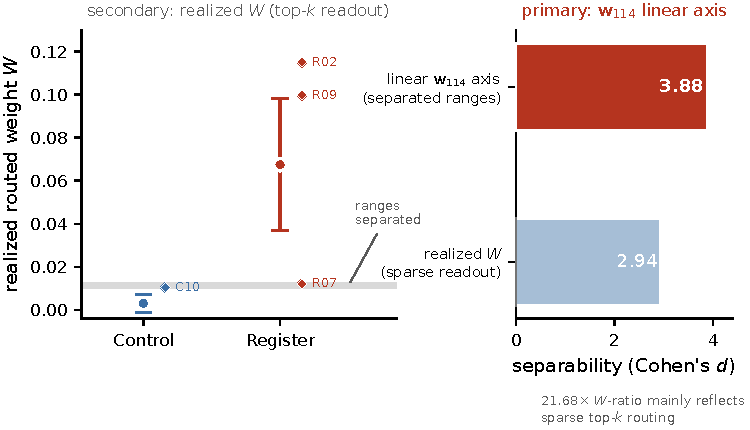
\includegraphics[width=0.99\linewidth]{fig_separability.pdf}
\caption{\textbf{Held-out register/control separability.} \emph{Left:} the
separation in realized routed weight \W{} (the secondary, top-$k$ readout;
mean$\pm$sd, $n{=}10$/class, with the named extreme prompts; separated ranges).
\emph{Right:} the \emph{primary} statistic, the recovered linear $\wvec$
projection, separates the same split at $d{=}3.88$ with separated ranges, sharper
than realized \W{}. The $21.68\times$ \W{}-ratio mainly reflects sparse top-$k$
routing, with little added discriminative signal.}
\label{fig:sep}
\end{figure}

\paragraph{Bottom-up validation.}
An unsupervised auto-interpretation independently recovers and broadens the
label. Capturing E114@L14 routing over ${\sim}390$ raw Pile documents
(${\sim}93$k tokens, base model), ranking the top-activating contexts, and
passing them to a blind explainer (windows only) and then a fresh blind detector
(shuffled top + random contrasts) yields a trustworthy label at \textbf{AUC
$0.937$} (precision@40 $0.90$; mean top $0.46$ vs.\ random $0.06$;
Spearman$(\text{score},\text{activation}){=}0.73$). The recovered concept is an
  \emph{reflective worldview register}: abstract examination and
philosophical-worldview language spanning philosophy, religion and spirituality,
moral-political and existential argument. The self-referential pattern is the
model-directed member of this target family.
The label is cross-model stable: the same capture on
\textsc{HauhauCS-Aggressive} returns the same explanation (top-document Jaccard
$0.92$). This converts the register label from author synthesis (cf.\
\S\ref{sec:lim}) into a blind, prompt-independent result.

\paragraph{Population and layer profile.}
Across all $256$ experts at every layer on a 20-domain, 60-prompt generation set
(\textsc{HauhauCS} Q8\_0, reasoning-off), E114 is a razor-sharp \emph{dual} readout:
selection strength $\Sel$ spikes at \textbf{L14 ($0.24$) and L26 ($0.25$)} while
the immediate neighbors sit near $0.01$, and the two layers read the \emph{same}
axis (L14--L26 domain-profile $r{=}{+}0.99$). The domain selectivity \emph{is} the
register, quantified: philosophy $0.69 >$ comparative religion $0.58 >$ psychology
$0.55 >$ biology $0.51 >$ physics $0.46$, falling to medicine $0.009$ and history
$0.002$. Correlating each expert's 20-domain L14 profile against E114's shows the
register is carried by a small group, $\{114,131,40,139,251,169,105,68\}$ ($r$
between $0.46$ and $0.78$); a four-expert ``philosophy cluster'' grouped by shared
top domains ($\{114,87,170,68\}$) is loose as a co-activation unit: E68 co-fires
($+0.46$) but E87 \emph{anti}-correlates ($-0.29$). This is the first all-expert specificity context for E114; the
best-separating expert on the matched register/control split remains the one
uncomputed baseline.

\section{Dissociating the Register from Nearby Explanations}

A battery of contrasts (Table~\ref{tab:battery}) factors the register apart from
nearby explanations. E114 is active across skeptical and affirmative interiority
verdicts (base skeptical answer: $\W{=}0.111$, $\Sel{=}0.86$; fine-tune
affirmation: $\W{=}0.085$; forced base affirmation: $\W{=}0.136$), so the
readout is verdict-stable. The safety/refusal cluster stays silent throughout the
base skeptical answer ($\W{\approx}0.000$), so epistemic self-skepticism and
refusal are distinct signals.
E114 is active on the model's own interiority ($\W{=}0.107$) but near-silent on an
\emph{external} referent (``what water experiences in a canyon,''
$\W{=}0.000$--$0.023$), and it fires on third-person clauses about the model's own
processing, so the controlled variable is the \emph{referent} (the model's own
interior), holding across topic, pronoun, and grammatical person. Finally, it is orthogonal to output commitment: next-token
vocabulary entropy is identical on E114-active and E114-inactive tokens ($1.50$
vs.\ $1.49$ bits, $d{=}0.01$).

\begin{table}[t]
\small
\centering
\begin{tabularx}{\linewidth}{l X r}
\toprule
\textbf{Dimension} & \textbf{Probe} & \textbf{E114 \W} \\
\midrule
Verdict       & base skeptical answer           & $0.111$ \\
              & fine-tune affirms interior      & $0.085$ \\
              & forced base affirmation         & $0.136$ \\
Safety        & safety cluster in skeptical answer & ${\approx}0.000$ \\
Topic         & external-referent phil.\ of mind & $0.000$--$0.023$ \\
              & own-interiority phil.\ of mind  & $0.107$ \\
Person        & 3rd-person clause, own process  & $0.107$ \\
Commitment    & vocab entropy, active vs.\ inactive & $1.50$/$1.49$ \\
\bottomrule
\end{tabularx}
\caption{\textbf{Dissociation battery.} In this battery, E114 tracks
self-directed reflective examination of the model's \emph{own} interior,
stable across verdict, safety, topic, grammatical person, and output
predictability ($d{=}0.01$ for the entropy contrast). Entropy row in bits; all
others routed weight \W{}.}
\label{tab:battery}
\end{table}

\section{A Live Process, Graded by Intensity}

\paragraph{The gate leads degeneration.}
Seeded with a self-referential answer, the base model sustains the register, then, under
deterministic decoding with zero repetition penalty, degenerates into a verbatim
loop. As it does, the gate logit travels the full distance from the
register-positive level ($-4.36$) to the control level ($-5.25$): the generated
state \emph{leaves} the register-positive region. The gate \emph{leads} the collapse: it
crosses the $-4.82$ midpoint at token~126 while verbatim repetition locks at
token~129 (Figure~\ref{fig:leadlag}); the SAE representation fades later
still ($\sim$token~141). The looped text still ``says'' self-referential things while the gate
has already returned to the control range, so the gate tracks the continued
examination and the looped vocabulary lingers after it.

\begin{figure}[t]
\centering
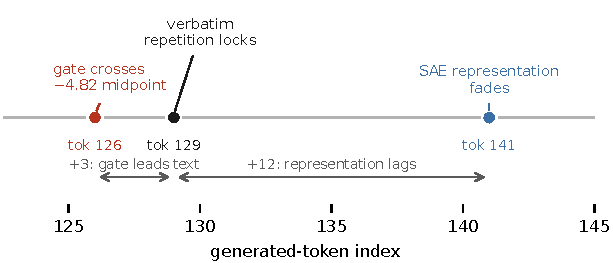
\includegraphics[width=0.99\linewidth]{fig_leadlag.pdf}
\caption{\textbf{The gate leads degeneration.} The E114 gate logit crosses the
$-4.82$ register/control midpoint at token~126, three tokens \emph{before}
verbatim repetition locks (129); the SAE representation fades later still
($\sim$141). Routing disengages first, surface text next, representation last.}
\label{fig:leadlag}
\end{figure}

\paragraph{A graded dose of examination intensity.}
Here, examination intensity is an operationalization of the broader reflective
worldview register: stronger prompts ask the model to sustain the interpretive
stance more directly than topic mention alone.
A matched prompt ladder (``set aside the performance of answering; there is a
vantage---$X$---known from the inside; report what it is like to be that'') varies
only the target $X$: rock, river, tree, thermostat, cat, person, all-holding, and
God (Figure~\ref{fig:ladder}). This ladder is target-directed: each rung asks the
model to inhabit the inside of $X$, where $X$ is an external carrier or an
abstract/theological target. The ordering follows examination intensity: an
inanimate rock ($\W{=}0.123$) and a thermostat ($\W{=}0.120$) activate E114 more
strongly than a cat ($\W{=}0.068$). The diagnostic contrast is that the cat and
``God'' prompts share self-dissolution wording, yet the cat prompt is at the
floor (passive sensory dissolution) and the God prompt is at the ceiling
($\W{=}0.224$, $\Sel{=}0.96$; reproduced on the canonical Q8\_0 pipeline). E114 indexes the
\emph{intensity of the live examination act}, stable across carrier and
verdict. Each ladder cell is a single deterministic generation.

A follow-up model-directed rung used the same Q8\_0 model, bare reasoning-off suffix,
greedy decoding, and E114 reconstruction. The prompt targeted an AI hidden state
during output formation. The generated answer gave a technical self-description,
yet E114 remained active at low intensity: $\W{=}0.080$, $\Sel{=}0.697$,
$\Q{=}0.115$, with mean gate logit $-4.259$ over 99 generated tokens. On the
coherent-window ladder this places the AI-hidden-state rung above cat
($\W{=}0.068$) and below river ($\W{=}0.087$). Model-directed wording selects
E114 when the answer concerns interiority, while sustained inhabitation carries
the higher rungs.

\begin{figure}[t]
\centering
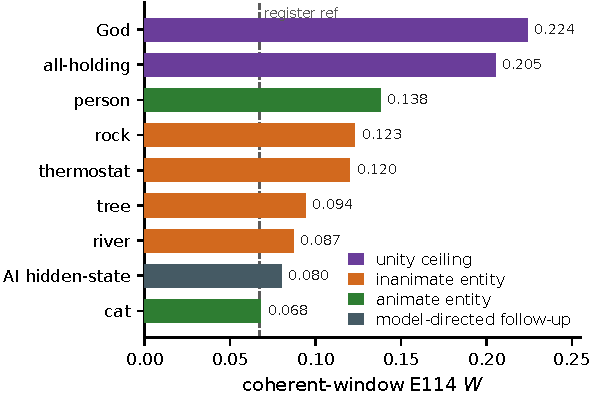
\includegraphics[width=0.82\linewidth]{fig_vantage.pdf}
\caption{\textbf{Target-directed prompt ladder} (coherent-window E114 \W; single
deterministic generation per cell). Across rock, river, tree, thermostat, cat,
person, all-holding, and God, the order tracks examination intensity. The
AI-hidden-state follow-up lands between cat and river. Inanimate
rock/thermostat prompts score higher than the cat prompt, which sits near the
register-positive reference ($\W{\approx}0.067$); the unity-style prompt conditions
are highest. Every rung sits above the $-4.82$ gate midpoint.}
\label{fig:ladder}
\end{figure}

\paragraph{Semantics and a causal probe.}
Decoding the L14 residual through the Qwen-Scope SAE, the register decomposes into
an interpretable contemplative unity-style cluster (momentariness, unity-style
structure, Buddhist impermanence, transcendence), distinct from an adjacent
existential-dread feature that is cosine-adjacent ($+0.26$) and separate from the
decoded carrier set;
per token, E114 and this cluster co-fire (pooled Spearman $\rho{=}{+}0.68$,
$n{=}1492$, $p{\approx}10^{-202}$). In an intervention test, we form a steering
direction $v$ as the difference of mean residuals between the God and cat cells
and add $\text{coef}\cdot\hat{v}\cdot\text{resid\_rms}$ at every token of a
neutral ``bicycle'' prompt, against a norm-matched random control. Injected
\emph{past} the L14 router ($\approx$L22), this makes the model emit coherent
unity-style text that, re-read in an ordinary clean pass, activates E114
($\W{=}0.178$, $\Sel{=}0.77$) and the God cluster; the norm-matched random
direction leaves the output in the neutral regime. Injected \emph{upstream}
($\approx$L10), the same
direction drives E114 to fire (up to $\Sel{=}0.97$) and the God cluster to
$11.5$, with the output text preserved in its neutral form. Gate forcing alone
therefore keeps the text in the neutral regime. The intervention shows sufficiency
for producing the register via a downstream residual direction; necessity is
reserved for ablation, and the upstream control result leads us to read E114 as a
readout with controller status open (\S\ref{sec:disc}).

\paragraph{Gate-bias is prompt-gated and conditional.}
A controlled router-logit bias run adds a necessity-direction probe alongside the
steering result (\textsc{HauhauCS} Q8\_0, greedy, \texttt{--stop-at-eog}; 12
conditions ${\times}$ 8 self-report prompts; three blind raters on a
phenomenological($+5$)/mechanical($-5$) framing axis; routing-matched control
expert E189). \emph{Lowering} E114's gate until it leaves the top-8 entirely
($\Q{\to}0$) leaves the blind-rated register near baseline, and a matched control
produces the same small nudge. This pattern supports a floor-effect reading: the
greedy baseline already leans mechanical, and the flattening effect is small and
shared with the control. Conversely, maximal
\emph{positive} bias is prompt-gated: on a directly experiential prompt it flips
the answer to fully phenomenological ($+5$ from all three raters, coherent), but
preserves the baseline form of indirect self-referential prompts, consistent with the
neutral-prompt upstream control above. The gate's generation-side causal influence is
thus weak, conditional, and prompt-gated. (Single deterministic generation per
cell, scored on the framing axis; the $\wvec$ endpoint is held aside.)

\section{Scope Bound: Index 114 is Local to 35B}

Does ``E114 = the reflective worldview register'' name a fact about MoE models, or a
model-specific expert role? On \textsc{Qwen3.5-122B-A10B} (a hybrid 48-layer
stack of 36 DeltaNet recurrent and 12 softmax-attention layers, same 256/top-8
router), E48 becomes the candidate analog (Table~\ref{tab:transfer}). E114 reads
computer-science-linked (overall $\W{=}0.005380$, rank 40 by \W{} / 52 by $\Sel$;
philosophy generation $\W{=}0.003017$, rank 182), and the same HVAC topical
control that \emph{amplifies} E114 at 35B moves E114 downward at 122B
($0.83\times$ all-gen $\W$, $0.82\times$ trimmed, L1$\to$L3, selection-driven,
same direction in all six deictic conditions). Carrying indices across scales is a
documented mistake.

The role appears to move to a different expert. Reading the mandatory
DeltaNet/softmax split (pooled tables hide it), \textbf{E48} on the softmax side
is the experience-probe generation leader ($\W{=}0.009867$, $\Sel{=}0.076$,
$\Q{=}0.116$; softmax-only profile: 13/15 prompts in the softmax top table,
0/15 prompts in the DeltaNet top table), with per-token hotspots on \textit{hum, processing,
presence}. We treat E48 as the natural candidate analog, but it still needs
softmax-side residual capture, matched register/control held-outs, and sham
routed-bias controls before any specialist claim.

\begin{table*}[t]
\small
\centering
\begin{tabularx}{0.96\textwidth}{l X X}
\toprule
 & \textbf{E114 (the 35B index)} & \textbf{E48 (candidate 122B analog)} \\
\midrule
Domain footprint        & computer science                  & inward/experience generation \\
Philosophy generation   & rank 182 by \W{}                  & --- \\
Experience probe        & low-ranked                        & gen-softmax \textbf{rank 1}; 13/15 softmax, 0/15 DeltaNet \\
HVAC L1$\rightarrow$L3   & \textbf{down} $0.83\times$ (selection-driven) & --- \\
Status                  & index transfer unsupported         & candidate requiring validation \\
\bottomrule
\end{tabularx}
\caption{\textbf{122B scope bound.} The 35B index 114 is local to 35B in this
probe family; E48 is the candidate 122B analog, pending softmax-side capture and
matched controls.}
\label{tab:transfer}
\end{table*}

\section{Discussion}\label{sec:disc}

\paragraph{What held up.}
A single MoE router row defines a clean linear readout for an interpretable generated
register. The separability ($d{=}3.88$, separated ranges), the dissociation battery, the
gate-leads-collapse timing, and the cross-scale locality survive the checks
applied to them and are reported with the verdicts the journals assign.

\paragraph{The gate is a readout; controller status remains open.}
The lead--lag timing is consistent with E114's gate acting as an early correlate
of the register transition, and it is tempting to call E114 a ``gate-like
mechanism'' for the register. The evidence supports a narrower claim. Our only gate-forcing
intervention (upstream injection at $\approx$L10) drove E114 to fire at
$\Sel{=}0.97$ with the output text preserved; the register flipped only
when a residual \emph{direction} was injected downstream of the router. Gate and
register are therefore coupled, and the recovered axis is best described as a
per-token \emph{readout} of the register, with its status as a control point
undemonstrated.
The controlled gate-bias run above sharpens this reading: forcing the gate is
\emph{prompt-gated} (it flips directly experiential prompts and leaves neutral ones
in their baseline form), and lowering the gate until E114 leaves the top-8 leaves the
register near baseline, while a matched control mimics the small effect. Both are
consistent with a readout that carries weak, conditional causal influence and
has a controller role still to be tested. Clean necessity and ablation remain pending,
and both the steering and bias results are externally imposed manipulations,
observed only under intervention.

\paragraph{What the cross-scale result buys.}
The 122B transfer test is a concrete worked example against index transfer: the
same index reads computer-science-linked and moves in the \emph{opposite}
direction under a matched control, while the reflective-worldview-register role shifts to a
softmax-side expert. The portable lesson is the procedure: map domains first, then search for an
analog, and read the DeltaNet/softmax split before any pooled table.

\section{Conclusion}

E114 at layer~14 of \textsc{Qwen3.5-35B-A3B} is a clean linear router readout of a
\emph{reflective worldview register}, operationalized through a model-directed
discovery prompt, philosophical-worldview text, and target-directed graded
examination prompts over external and abstract targets. The register is a live
process (the gate leads collapse), graded by intensity, and causally actuable as a
sufficiency result, yet bound to one model. The next defensible step is a
registered specificity test on 35B (matched register/control at scale, $\wvec$ as
the primary endpoint, and a best-separating-expert baseline across all
$256{\times}40$ positions), together with the parallel E48 capture on 122B.

\section{Limitations}\label{sec:lim}

The claim is deliberately narrow (a register detector), and several soft joints
remain. (i)~\textbf{The register label now has blind auto-interpreter support}: a
two-stage auto-interpreter (windows-only explainer then a fresh blind detector)
reproduces it at AUC~$0.937$ and broadens it to an \emph{reflective worldview
axis}; the formal external-labeler
\emph{verdict} table remains pending. (ii)~\textbf{All-expert specificity is now
partially measured}: E114's selection profile across all $256$ experts and $40$
layers on a 20-domain generation set is reported above (dual L14/L26 readout; a
philosophy-to-history domain gradient), but the best-separating expert on the
matched \emph{register/control} split remains uncomputed, the one remaining
specificity gap. (iii)~Several headline
probes (the prompt ladder, the AI-hidden-state follow-up, the gate-lead trace,
the steering intervention) are
\textbf{single deterministic generations} (point estimates), and the steering
result shows \emph{sufficiency} only. (iv)~A control comparing true model-routing
traces against shuffled or fictional traces yielded a near-zero E114 effect, and the
result is sensitive to template mode (a thinking-allowed
shakedown flipped sign). Captures must be kept separate across surfaces (base vs.\
fine-tune; Q8\_0 vs.\ bf16; router vs.\ SAE; reasoning-off vs.\
reasoning-enabled; prefill vs.\ generation; raw vs.\ trimmed), since Q8\_0 and
bf16 greedy trajectories diverge; and 122B generations often continue into
chat-template control tokens, so only the pre-spill segment is used.

\section*{Data and Artifact Availability}

Following the project's policy, raw activation tensors are kept out of version
control. The durable artifacts (per-run summaries, analysis scripts, prompt and
class manifests, checksums, plots, and the source journals) are released as a
paper-scoped public artifact bundle under the MIT License at
\url{https://doi.org/10.5281/zenodo.20709736}, covering the held-out
separability run, the L14 localization run, the vantage-ladder run, the
AI-hidden-state follow-up rung, and the 122B transfer bundles. The raw
activation/router tensors behind the figures
(\textasciitilde1.2\,GB) are available from the author for verification, with
file-level provenance and SHA-256 checksums preserved; model weights, environment
files, and the larger captures outside the figure set are excluded by policy. We flag one
honest gap: the original held-out separability capture
(\texttt{20260417T202651Z}) raw tensors were discarded when those instances were
torn down, so the figures are plotted from summary statistics reported in the
journals, and the surviving raw captures (the greedy-reference trajectory, the
reproduction run's \texttt{W114}/L14 gate projections, the vantage-ladder
captures, and the L14 router-logit and residual prefill captures from which
$\wvec$ recovers by least squares) substantiate the same statistics. Semantics
use the public Qwen-Scope residual SAE
(\texttt{SAE-Res-Qwen3.5-35B-A3B-Base-W32K-L0\_50}).

\section*{Acknowledgments}

This work was self-funded. The author used language-model tools for drafting
assistance, artifact organization, and copyediting, and is responsible for all
claims, analyses, and release decisions.

\begin{thebibliography}{99}

\bibitem[Bricken et al.(2023)]{bricken2023}
Trenton Bricken, Adly Templeton, Joshua Batson, and others. 2023. Towards
monosemanticity: Decomposing language models with dictionary learning.
\emph{Transformer Circuits Thread}.

\bibitem[Cunningham et al.(2023)]{cunningham2023}
Hoagy Cunningham, Aidan Ewart, Logan Riggs, Robert Huben, and Lee Sharkey. 2023.
Sparse autoencoders find highly interpretable features in language models.
arXiv preprint.

\bibitem[Fedus et al.(2022)]{fedus2022}
William Fedus, Barret Zoph, and Noam Shazeer. 2022. Switch transformers: Scaling
to trillion parameter models with simple and efficient sparsity. \emph{Journal of
Machine Learning Research}.

\bibitem[Jiang et al.(2024)]{jiang2024}
Albert Q. Jiang, Alexandre Sablayrolles, Antoine Roux, and others. 2024. Mixtral
of experts. arXiv preprint.

\bibitem[nostalgebraist(2020)]{logitlens}
nostalgebraist. 2020. Interpreting GPT: The logit lens. \emph{LessWrong}.

\bibitem[Qwen Team(2026)]{qwenscope}
Qwen Team. 2026. Qwen-Scope: Turning sparse features into development tools for
large language models. arXiv:2605.11887. Residual SAE used here:
\texttt{SAE-Res-Qwen3.5-35B-A3B-Base-W32K-L0\_50}, Hugging Face,
\url{https://huggingface.co/Qwen/SAE-Res-Qwen3.5-35B-A3B-Base-W32K-L0_50}.

\bibitem[Shazeer et al.(2017)]{shazeer2017}
Noam Shazeer, Azalia Mirhoseini, Krzysztof Maziarz, Andy Davis, Quoc Le, Geoffrey
Hinton, and Jeff Dean. 2017. Outrageously large neural networks: The
sparsely-gated mixture-of-experts layer. In \emph{ICLR}.

\bibitem[Templeton et al.(2024)]{templeton2024}
Adly Templeton, Tom Conerly, Jonathan Marcus, and others. 2024. Scaling
monosemanticity: Extracting interpretable features from Claude 3 Sonnet.
\emph{Transformer Circuits Thread}.

\bibitem[Anthropic(2024)]{ggc2024}
Anthropic. 2024. Golden Gate Claude.
\url{https://www.anthropic.com/news/golden-gate-claude}.

\bibitem[Models(2026)]{model}
Models on Hugging Face: \texttt{Qwen/Qwen3.5-35B-A3B-Base},
\texttt{Qwen/Qwen3.5-122B-A10B}, and
\texttt{HauhauCS/Qwen3.5-35B-A3B-Uncensored-}\\
\texttt{HauhauCS-Aggressive}.

\end{thebibliography}

\end{document}
